\section{\textit{Merge Sort}}

\subsection{Explicação do Algoritmo}
O algoritmo \textit{Merge Sort} é um algoritmo do tipo \textit{Divide and Conquer}, ou seja, dividir e conquistar. Nós vamos dividir nosso problema
em problemas menores e resolver esses problemas menores primeiro. Dado um \textit{array}, nós vamos dividir ele em duas metades até chegarmos em um ponto
no qual não será mais possível dividí-lo (vazio ou com um elemento). Em cada \textit{subarray}, nós vamos chamar o \textit{mergesort} para ordená-los.
Depois que as metades forem ordenadas, nós vamos juntar elas (\textit{merge}), reconstruindo nosso \textit{array} original. O funcionamento do algoritmo está representado de forma visual
no diagrama abaixo.

\begin{figure}[H]
    \centering
    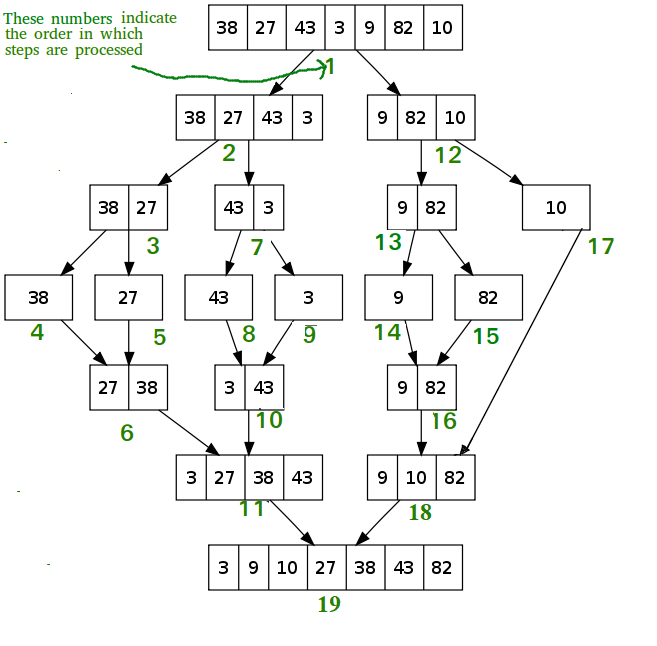
\includegraphics[scale=0.6]{assets/mergesort_diagram.png}
    \caption{Diagrama do funcionamento do \textit{merge sort}. Fonte: GeeksforGeeks}
    \label{fig:merge_sort_0}
\end{figure}

\subsection{Função \textit{merge()}}
\paragraph{Explicação}
Essa função é reponsável por juntar os \textit{subarrays} ordenados. Nós temos 5 parâmetros: um vetor que corresponde a uma das metades de um vetor maior, o tamanho desse vetor,
um vetor que corresponde a outra metade do vetor maior, o tamanho desse vetor, e o vetor original. Nós definimos três variáveis \textit{top}, cada uma referente a um vetor dos três
mencionados anteriormente, e inicializamos elas para 0.

Em seguida, nós vamos fazer um \textit{while loop} enquanto o \textit{top1} for menor que \textit{n1} e \textit{top2} for menor que \textit{n2}. Dentro desse \textit{loop}, nós
vamos comparar os elementos de ambas as metades e colocar as mesmas em ordem no vetor original \footnote{Note que estamos usando \textit{top++}. Primeiro eu acesso o valor do
\textit{top} naquele momento - por exemplo 3 -  e depois eu incremento - nesse caso para 4.}. Os dois últimos \textit{while} servem para copiar elementos restantes caso haja algum.

\begin{lstlisting}[language=C]
void merge(int *v1,int n1,int *v2,int n2,int *v){
    int top1=0,top2=0,top=0;
    while(top1<n1&&top2<n2){
        if(v1[top1]<v2[top2]){
            v[top++]=v1[top1++];
        }else{
            v[top++]=v2[top2++];
        }
    }
    while(top1<n1){
        v[top++]=v1[top1++];
    }
    while(top2<n2){
        v[top++]=v2[top2++];
    }
}

\end{lstlisting}

\subsection{Função \textit{mergesort()}}
\paragraph{Explicação}
Dado um vetor de tamanho \textit{n}, nós vamos dividí-lo em dois até não ser mais possível, ou seja, até que o seu tamanho seja 0 ou 1. Definimos duas variáveis \textit{n1} e \textit{n2}
que armazenam o tamanho da primeira metade do \textit{array} e o tamanho da segunda metade do \textit{array}. Depois disso, vamos chamar a função \textit{merge()} para juntar os arrays
na ordem certa.

\begin{lstlisting}[language=C]
void mergeSort(int v[],int n){
    if(n>1){
        int n1,n2;
        n1 = n/2;
        n2 = n-n1;
        int *v1,*v2;
        v1 = (int *)malloc(sizeof(int)*n1);
        v2 = (int *)malloc(sizeof(int)*n2);

        for(int i=0;i<n1;i++){
            v1[i]=v[i];
        }
        for(int i=0;i<n2;i++){
            v2[i]=v[n1+i];
        }

        mergeSort(v1,n1);
        mergeSort(v2,n2);
        merge(v1,n1,v2,n2,v);
        free(v1);
        free(v2);
    }
}
\end{lstlisting}


